% Noise Padifier - user manual (English; French version: manuel.tex).
% pdflatex manual.tex (three passes); figures: python3 figures.py (doc/fig_*_en.pdf).
% Copyright (C) 2026 Padifier authors - SPDX-License-Identifier: GPL-3.0-or-later
\documentclass[a4paper,11pt]{article}
\usepackage[T1]{fontenc}
\usepackage[utf8]{inputenc}
\usepackage[english]{babel}
\usepackage{lmodern}
\usepackage{microtype}
\usepackage[margin=2.3cm]{geometry}
\usepackage{amsmath,amssymb}
\usepackage{graphicx}
\usepackage{booktabs}
\usepackage{array}
\usepackage{tabularx}
\usepackage{xcolor}
\usepackage{tikz}
\usetikzlibrary{arrows.meta,positioning,fit,calc}
\usepackage{enumitem}
\usepackage[hidelinks]{hyperref}

\definecolor{amber}{HTML}{96691A}
\definecolor{violet}{HTML}{6246AA}
\definecolor{ink}{HTML}{26203A}
\definecolor{paper}{HTML}{F4F2F8}

\newcommand{\ctl}[1]{\textsf{\textbf{#1}}}   % name of an element of the interface
\newcommand{\dB}{\,dB}
\newcommand{\dBFS}{\,dBFS}
\setlist{itemsep=1pt,topsep=3pt}
\emergencystretch=3em
\graphicspath{{./}{captures/}}

\title{\textsf{NOISE} \textcolor{violet}{\textbf{PADIFIER}}\\[4pt]
\large User manual and description of the algorithm}
\author{Version 1.1.0}
\date{}

\begin{document}
\maketitle

\begin{center}
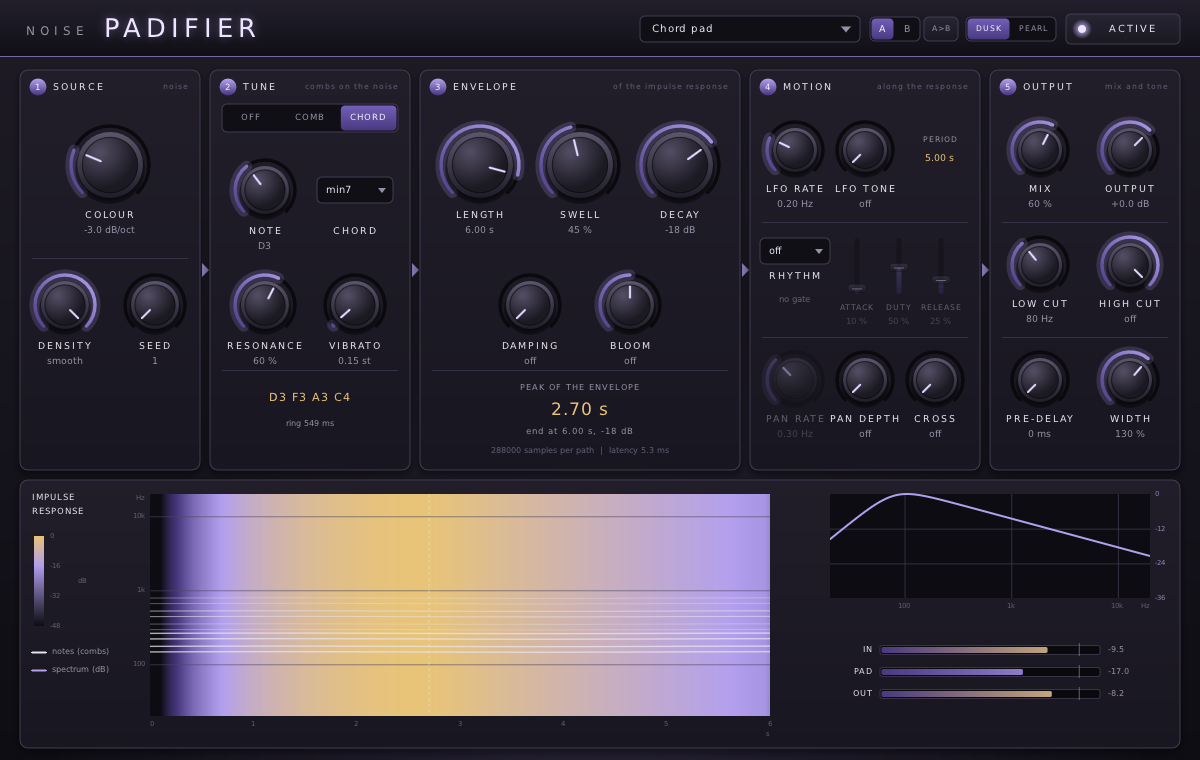
\includegraphics[width=0.92\textwidth]{capture_dusk.png}
\end{center}

\newpage
\tableofcontents
\newpage

% ==============================================================================================
\section{Overview}

Noise Padifier turns any sound into a pad. The signal is convolved with an impulse response made
of \textbf{noise} under an adjustable \textbf{envelope}, 0.1 to 10\,s long: every note, every
attack, is smeared over the whole length of that response. Since noise contains every frequency,
the timbre of the source is kept (its harmonics stay where they are) but its shape in time is
gone: a short note becomes a sustained sound that rises and dies away along the envelope
(figure~\ref{fig:pad}).

The noise itself is shaped: its colour (from brown to violet), its density (from smooth noise to a
cloud of grains), a tuning on a note or a chord by comb filters, an envelope that depends on
frequency (highs that die sooner, lows that bloom later), an LFO, a rhythm on the tempo, a stereo
motion and a true crossed stereo. All these treatments act \textbf{along the response}: they are
computed once, when the response is built, and cost nothing during playback.

\begin{figure}[htbp]
\centering
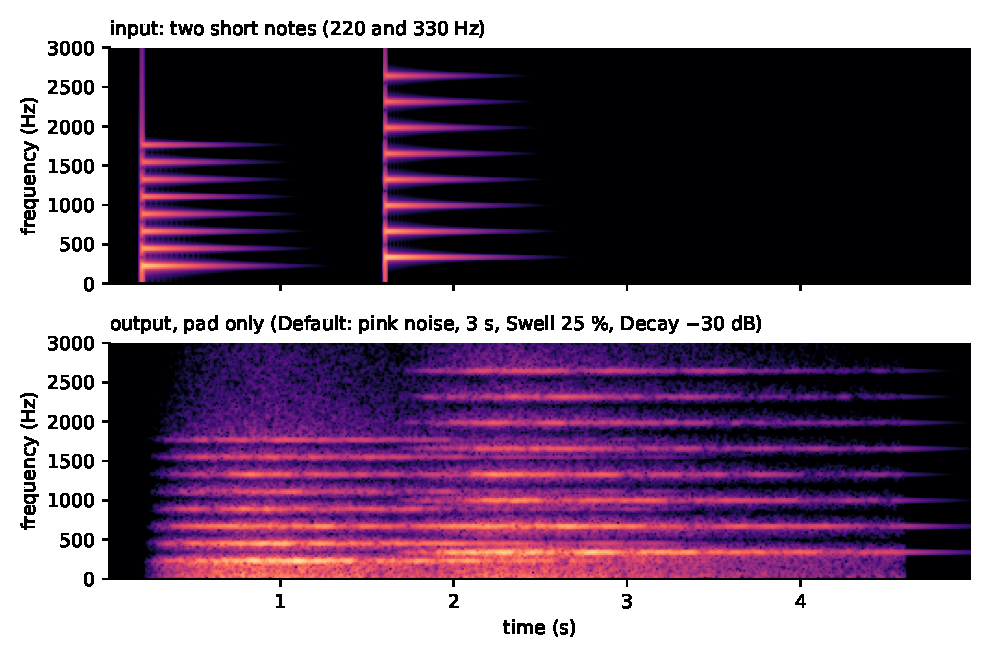
\includegraphics[width=\textwidth]{fig_pad_en.pdf}
\caption{Two short notes (top), what the Default preset makes of them (middle: each note lasts
3\,s, rises in 0.75\,s, then decays), and the Chord pad preset (bottom: the pad is tuned to a
D minor 7 chord).}
\label{fig:pad}
\end{figure}

Around the convolution: pre-delay, low cut and high cut on the pad, stereo width, mix with the dry
sound, output gain, presets, A/B comparison.

\paragraph{Formats.} VST3 and CLAP for 64-bit Windows; VST3, CLAP and LV2 for Linux. The plugin is
stereo (two inputs, two outputs). Its \textbf{latency is 256 samples} (5.3\,ms at 48\,kHz),
reported to the host, which compensates it.

\paragraph{Licence.} GPL 3 or later (file \texttt{COPYING}). The interface and the plugin formats
rely on DPF (ISC licence); the Fourier transforms on pffft by Julien Pommier (FFTPACK licence,
BSD-like).

% ==============================================================================================
\section{Installation}

\paragraph{Windows.} Run the installer \texttt{Noise-Padifier-1.1.0-setup.exe}. It installs the
VST3 (required) and, if ticked, the CLAP and the user manuals (English and French), then adds an
uninstaller (``Apps and features''). By hand, copy:
\begin{itemize}
\item the \texttt{noise\_padifier.vst3} folder to \verb|C:\Program Files\Common Files\VST3\|;
\item \texttt{noise\_padifier.clap} to \verb|C:\Program Files\Common Files\CLAP\|.
\end{itemize}

\paragraph{Linux.} Copy \texttt{noise\_padifier.vst3} to \verb|~/.vst3/|,
\texttt{noise\_padifier.clap} to \verb|~/.clap/| or \texttt{noise\_padifier.lv2} to
\verb|~/.lv2/|.

Then rescan the plugins in your host. The uninstaller leaves the preferences and the presets of
the user in place (section~\ref{sec:files}).

% ==============================================================================================
\section{Getting started in one minute}

\begin{enumerate}
\item \textbf{As an insert} on a track: the \ctl{Default} preset is loaded (pink noise, 3\,s,
  Mix 50\,\%). \textbf{On an auxiliary send}: choose \ctl{Send (100 \% wet)}, which returns the
  pad only.
\item Set the length of the pad with \ctl{LENGTH}, its rise with \ctl{SWELL} and its end with
  \ctl{DECAY}; the map at the bottom shows the resulting response.
\item Choose the colour with \ctl{COLOUR}: to the left darker and warmer, to the right brighter;
  refine with \ctl{LOW CUT} and \ctl{HIGH CUT}.
\item For a tuned pad: \ctl{TUNE} on \ctl{COMB} (one note) or \ctl{CHORD} (a chord), then
  \ctl{NOTE}, \ctl{CHORD} and \ctl{RESONANCE}.
\item For motion: \ctl{RHYTHM} (pulse on the tempo), \ctl{PAN DEPTH} (stereo swing),
  \ctl{VIBRATO} or \ctl{LFO TONE}.
\item Dose with \ctl{MIX}. The presets show each treatment.
\end{enumerate}

\section{The interface}

The window (1200 × 760 points, resizable with its proportions kept, sharp on high-density screens)
reads from left to right in the order of the signal: five numbered sections linked by arrows,
then, at the bottom, the map of the response, the spectrum of the pad and the meters. Every element
has a tooltip on hover; for a knob, its title gives the detailed value. A knob without effect with
the other settings is drawn faint (for example NOTE when TUNE is OFF); it can still be used.

\begin{center}
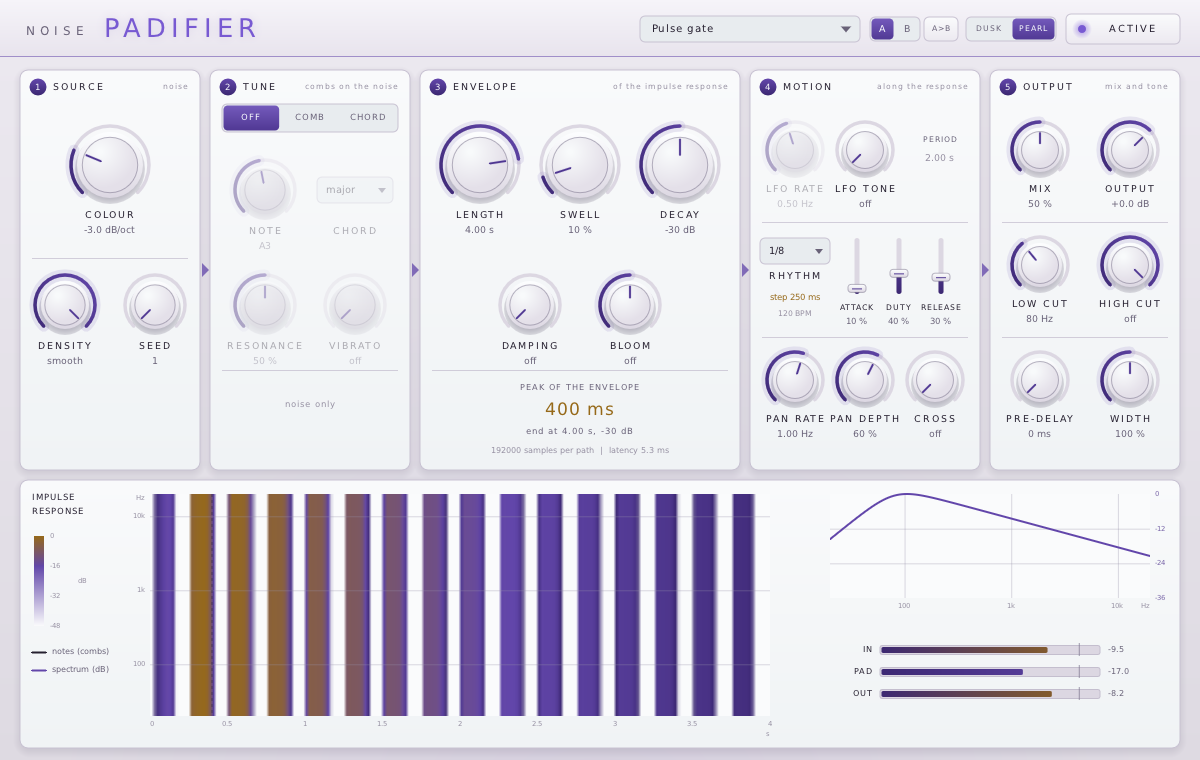
\includegraphics[width=0.85\textwidth]{capture_pearl.png}\\[2pt]
\small Light theme \ctl{PEARL}, Blooming preset, tooltip of BLOOM.
\end{center}

\subsection{Header}
\begin{description}
\item[Presets.] Drop-down list: a click opens it; it shows the factory presets (\ctl{FACTORY}), a
  line, your presets (\ctl{USER}, in alphabetical order), a line, then \ctl{Save current
  settings\ldots}. The current preset is marked with a dot; ``*'' after its name means a setting
  was changed since it was loaded. The mouse wheel over the closed box steps to the next or
  previous preset. Details in section~\ref{sec:presets}.
\item[A | B and A>B.] Two sets of settings to compare: a click on \ctl{A} or \ctl{B} switches (the
  set you leave is kept, the other one is loaded; on its first visit, B starts as a copy of A).
  \ctl{A>B} (or \ctl{B>A}) copies the current set into the other. Both sets are saved with the
  project.
\item[DUSK | PEARL.] Dark or light theme, with no effect on the sound; it is a preference of the
  computer, shared by all instances and all projects.
\item[ACTIVE / BYPASSED.] The bypass declared to the host (section~\ref{sec:smoothing}).
\end{description}

\subsection{Section 1: SOURCE}
\ctl{COLOUR}, \ctl{DENSITY} and \ctl{SEED}: the noise to start from.

\subsection{Section 2: TUNE}
The \ctl{OFF | COMB | CHORD} selector, then \ctl{NOTE}, the \ctl{CHORD} list, \ctl{RESONANCE} and
\ctl{VIBRATO}. Below: the note and its frequency (or the notes of the chord) and the ring time of
the combs.

\subsection{Section 3: ENVELOPE}
\ctl{LENGTH}, \ctl{SWELL}, \ctl{DECAY}, \ctl{DAMPING} and \ctl{BLOOM}. Below: the time of the peak of
the envelope (at 125\,Hz and 8\,kHz when Bloom is on), the end of the response and its level (and
at 8\,kHz with Damping), the number of samples per path and the latency.

\subsection{Section 4: MOTION}
Three rows: the LFO (\ctl{LFO RATE}, \ctl{LFO TONE}, and its period), the rhythm (the \ctl{RHYTHM} list
and the length of a step at the tempo of the host, then three vertical faders \ctl{ATTACK},
\ctl{DUTY} and \ctl{RELEASE}), the stereo (\ctl{PAN RATE},
\ctl{PAN DEPTH}, \ctl{CROSS}).

\subsection{Section 5: OUTPUT}
\ctl{MIX}, \ctl{OUTPUT}, \ctl{LOW CUT}, \ctl{HIGH CUT}, \ctl{PRE-DELAY} and \ctl{WIDTH}.

\subsection{Map, spectrum and meters}
\begin{itemize}
\item on the left, the \textbf{time-frequency map} of the response: time from 0 to Length from
  left to right, frequency from 20\,Hz to 20\,kHz from bottom to top, level in colour (0 to
  $-48$\dB, scale on the left). It shows the envelope, Damping, Bloom, LFO TONE and the gate of
  RHYTHM; the light lines are the notes of the combs (harmonics with COMB, the notes of the chord
  and two harmonics with CHORD), with their vibrato; dashed, the peak of the envelope. The colour
  of the noise is not on it: it is on the spectrum;
\item on the right, the \textbf{spectrum of the pad}: colour of the noise and filters, in dB, the
  highest point at 0\dB;
\item below, three peak meters: \ctl{IN} (input), \ctl{PAD} (pad alone, after the filters and
  Width, before the mix), \ctl{OUT} (output), in dBFS; after a peak, the display falls back with a
  time constant of 0.25\,s.
\end{itemize}

\subsection{Using the knobs}
\begin{itemize}
\item drag vertically; \textsf{Shift} for fine adjustment;
\item mouse wheel (\textsf{Shift}: fine);
\item double-click or \textsf{Ctrl}+click: default value;
\item faders (ATTACK, DUTY, RELEASE): drag vertically, the cap follows the mouse (\textsf{Shift}:
  fine); wheel, double-click and right-click as for the knobs;
\item whole-number settings (NOTE, SEED): one wheel notch per value;
\item \ctl{CHORD} and \ctl{RHYTHM} lists: a click opens the list of values (the current one is
  marked with a dot), a click chooses one, \textsf{Escape} or a click elsewhere closes it; the
  wheel over the closed box steps to the next or previous value;
\item right-click: type the value (\textsf{Enter} confirms, \textsf{Escape} cancels; a comma is
  accepted as the decimal separator).
\end{itemize}

% ==============================================================================================
\section{The settings}

\begin{center}
\small
\begin{tabularx}{\textwidth}{@{}l l l X@{}}
\toprule
Setting & Range & Default & Role \\
\midrule
\multicolumn{4}{@{}l}{\textsf{1 SOURCE}} \\
Colour & $-6$--+6\dB/oct & $-3$ & slope of the spectrum of the noise ($-3$: pink) \\
Density & 10--10\,000 /s & smooth & impulses per second (at the maximum: smooth noise) \\
Seed & 1--99 & 1 & draw of the noise \\
\multicolumn{4}{@{}l}{\textsf{2 TUNE}} \\
Tune & off, comb, chord & off & comb on the note, or combs on a chord \\
Note & C1--C7 & A3 & note of the comb, root of the chord \\
Chord & 9 chords & major & kind of chord \\
Resonance & 0--100\,\% & 50\,\% & ring time of the combs (20\,ms to 5\,s) \\
Vibrato & 0--12 semitones & 0 & depth of the LFO on the note \\
\multicolumn{4}{@{}l}{\textsf{3 ENVELOPE}} \\
Length & 0.1--10\,s & 3\,s & length of the response \\
Swell & 0--100\,\% & 25\,\% & rise of the envelope, as a part of the length \\
Decay & $-60$--0\dB & $-30$\dB & level of the envelope at the end \\
Damping & 0--12\dB/oct & 0 & loss of the highs at the end \\
Bloom & $-100$--+100\,\% & 0 & shift of the peak with frequency \\
\multicolumn{4}{@{}l}{\textsf{4 MOTION}} \\
LFO rate & 0.05--10\,Hz & 0.5\,Hz & rate of the LFO (vibrato, colour) \\
LFO tone & 0--6\dB/oct & 0 & depth of the LFO on the colour \\
Rhythm & off, 1/1--1/32 & off & gate on the tempo (dotted, triplets) \\
Attack & 0--100\,\% & 10\,\% & rise at the start of each step \\
Duty & 5--100\,\% & 50\,\% & open part of each step \\
Release & 0--100\,\% & 25\,\% & fall after the open part \\
Pan rate & 0.05--10\,Hz & 0.3\,Hz & rate of the stereo motion \\
Pan depth & 0--100\,\% & 0 & depth of the stereo motion \\
Cross & 0--100\,\% & 0 & true stereo: left-right crossings \\
\multicolumn{4}{@{}l}{\textsf{5 OUTPUT}} \\
Mix & 0--100\,\% & 50\,\% & part of the pad (constant power) \\
Output & $-24$--+12\dB & 0\dB & gain of the whole output \\
Low cut & 20\,Hz (off)--1\,kHz & off & 12\dB/octave high-pass on the pad \\
High cut & 1--20\,kHz (off) & off & 12\dB/octave low-pass on the pad \\
Pre-delay & 0--500\,ms & 0 & delay of the pad \\
Width & 0--200\,\% & 100\,\% & stereo width of the pad \\
Bypass & on/off & off & unprocessed (delayed) input, 10\,ms crossfade \\
\bottomrule
\end{tabularx}
\end{center}

\subsection{Source}

\paragraph{Colour.} Slope of the spectrum of the noise, in decibels (of power) per octave: $-6$,
brown noise, dark and deep; $-3$, pink noise (the same energy per octave), warm and full, close to
the balance of a reverb; 0, white noise, bright and airy, whose hiss is more audible in the highs;
$+3$ blue and $+6$ violet, higher and higher. Figure~\ref{fig:spectrum}.

\paragraph{Density.} At the maximum, the noise is smooth (Gaussian). Below, it is a sparse noise
(velvet noise): one impulse of random sign, at a random place, in each interval of 1/Density
second. At a few thousand per second it still sounds smooth; at a few tens, each sound is repeated
as a cloud of distinct grains or echoes.

\paragraph{Seed.} The noise comes from a pseudo-random generator: each value of Seed gives another
noise of the same kind. The differences are details (the ``grain'', a few frequencies a little more
or a little less present); the same value always gives exactly the same response, on any computer.

\subsection{Tune}

\paragraph{Tune.} \ctl{OFF}: noise only. \ctl{COMB}: the noise goes through a comb filter tuned to
NOTE; its resonances are the harmonics of the note, and the pad takes the colour of a string or a
pipe on that note. \ctl{CHORD}: one comb per note of the chord, summed. The convolution creates no
frequency absent from the input: the pad brings out what the source contains near these notes; a
rich source (noise, percussion, dense chord) gives a clearly tuned pad, an isolated note far from
the chord gives little sound.

\paragraph{Note.} Note of the comb, or root of the chord, from C1 (32.7\,Hz) to C7 (2093\,Hz),
A4 = 440\,Hz.

\paragraph{Chord.} major, minor, sus2, sus4, fifth (fifth and octave), maj7, min7, dom7, octaves
(three octaves of the note).

\paragraph{Resonance.} Ring time of the combs ($-60$\dB), from 20\,ms at 0\,\% to 5\,s at 100\,\%
(exponential law): low, a light tint; high, clear, almost sinusoidal notes.

\paragraph{Vibrato.} Depth, in semitones, of the LFO on the note of the combs; its rate is LFO
RATE. Like every motion, it starts at the attack of each sound (section~\ref{sec:lfo}).

\subsection{Envelope}

\paragraph{Length.} Length of the response, hence of the smearing: a few hundred milliseconds
thicken the sound (smear); several seconds make a pad. Logarithmic knob.

\paragraph{Swell.} Time of the peak of the envelope, as a percentage of the length. At 0, the pad
starts with the sound; at 25\,\% of a 3\,s response, it rises for 0.75\,s; at 100\,\%, it rises over
the whole response and then stops short (a ``reverse reverb'' effect).

\paragraph{Decay.} Level of the envelope at the end of the response, after the peak, along a
straight line in decibels: at $-60$\dB, the pad dies away like a reverb; at 0\dB, it stays at the
same level to the end (a held pad, cut by a fade of 20\,ms at most). Figure~\ref{fig:envelopes}.

\paragraph{Damping.} The highs die sooner than the lows, as in a room: at the end of the response,
each octave above 250\,Hz loses Damping decibels more than Decay (with 6\dB/oct and Decay
$-30$\dB, 8\,kHz ends at $-60$\dB). The pad gets darker as it dies away.

\paragraph{Bloom.} The peak of the envelope moves with frequency, by at most half the length over
four octaves on either side of 1\,kHz: positive, the highs arrive later (the pad opens up);
negative, the lows arrive later (it warms up).

\subsection{Motion}\label{sec:lfo}

\paragraph{Motion along the response.} The LFO, the rhythm and the stereo motion are written into
the response: they start at the attack of each sound, not on the time of the song. On spaced
notes, each one makes the same motion; on dense playing, the motions of the successive notes
overlap with an offset and soften. A response lasts 10\,s at most: a slow LFO only makes one or two
cycles per note.

\paragraph{LFO rate, LFO tone.} Rate of the LFO (a sine starting from 0 at the attack), shared by
the vibrato of the combs and the colour; LFO TONE swings the slope of the spectrum by $\pm$ its
value: the pad gets brighter and darker.

\paragraph{Rhythm, Attack, Duty, Release.} A gate cuts the response into steps of the chosen
division (1/1 to 1/32, dotted, triplets) at the tempo of the host (120\,BPM if it gives none). Each
step rises during Attack ($\sin^2$ curve), stays open until the end of Duty, then falls during
Release ($\cos^2$ curve). Attack and Release are in percent of the step, so that the shape follows
the tempo; their times are shown in the tooltip. Attack is part of Duty (bounded by it); Release
comes after and may run into the next step, the gate then taking the larger of the two levels (no
step down). Each edge lasts at least 1\,ms.
With a short Attack, Release and Duty, each sound comes back as separate bursts, like rhythmic
echoes; with long edges, the pad breathes or undulates (Duty 100\,\% and a non-zero Attack: an
amplitude modulation at the rate of the step). A change of tempo makes the response again.

\paragraph{Pan rate, Pan depth.} The pad swings between left and right: at 100\,\%, each side fades
out in turn (figure~\ref{fig:stereo}).

\paragraph{Cross.} True stereo: sets how much each input also feeds the pad on the opposite
side.

\emph{Without Cross (0)}, each side is processed on its own: left output = left input convolved
with a noise, right output = right input convolved with another, independent noise. The pad keeps
the position of the source: a sound placed hard left gives a pad hard left, nothing on the right.

\emph{With Cross}, each input also reaches the other side through a third and a fourth noise,
independent too:
\[
\text{output}_L = \cos\!\left(c\,\tfrac{\pi}{4}\right) (x_L * h_{LL})
               + \sin\!\left(c\,\tfrac{\pi}{4}\right) (x_R * h_{RL}),
\qquad c = \text{Cross} / 100,
\]
and likewise on the right. At 50\,\%, the direct path is at $-0.7$\dB{} and the crossed path at
$-8.3$\dB; at 100\,\%, both are at $-3$\dB: a sound placed hard left gives a pad of the same level
on both sides, and the pad fills the whole width whatever the position of the source. This is how
a real room behaves (a ``true stereo'' reverb), where a sound on the left resonates everywhere.

What Cross does not change:
\begin{itemize}
\item \textbf{the level}: for an input with independent channels, the energy of each output stays
  the same ($\cos^2 + \sin^2 = 1$);
\item \textbf{the width}: the four noises are independent, the two outputs stay decorrelated; the
  pad stays wide, it does not become mono;
\item \textbf{a mono source} (the same signal on the left and on the right): the output was
  already wide and balanced without Cross; Cross then only changes the draw of the noise, not the
  image. It is only useful for stereo sources whose two sides differ: instruments placed left or
  right, stereo drum recordings, stereo mixes sent to an auxiliary send.
\end{itemize}

\emph{Difference with Width}: Width acts afterwards on the pad already made; at 0\,\%, it makes it
mono (a pad placed on the left ends up in the centre, but narrow). Cross spreads the pad to both
sides while keeping it wide. The two can be combined.

\emph{Cost}: four convolutions instead of two, about twice the computation (4.5\,\% of one core
instead of 2.2\,\% at 48\,kHz for a 10\,s response) and the memory, and a slightly longer rebuild;
only when Cross is above 0. The stereo motion (Pan) is applied afterwards, output by output.

\emph{When to use it}: on an auxiliary send that receives sources placed left or right, when a pad
confined to one side sounds artificial. Leave it at 0 to keep the position of the source in the
pad, for a mono source, or to save computation.

\subsection{Output}

\paragraph{Mix.} Constant-power mix of the dry sound and the pad: pad $= \sin(\frac{\pi}{2}\,m)$,
dry $= \cos(\frac{\pi}{2}\,m)$, $m$ = Mix / 100 (figure~\ref{fig:mix}). At 50\,\%, both are at
$-3$\dB; at 100\,\%, only the pad remains (auxiliary send).

\paragraph{Output.} Gain of the whole output (dry and pad), after the mix.

\paragraph{Low cut, High cut.} Second-order Butterworth filters (12\dB{} per octave) on the pad
alone: Low cut between 60 and 200\,Hz keeps the low end of pink and brown noise out of the bottom
of the mix; High cut softens the pad and removes the high hiss. Logarithmic knobs; at their ends
(``off''), the filter is removed.

\paragraph{Pre-delay.} Delays the pad, by 0 to 500\,ms: it starts after the dry sound. A change
crossfades from the old delay to the new one in 30\,ms.

\paragraph{Width.} Stereo width of the pad alone: 0\,\% makes it mono, 100\,\% leaves it as it is,
200\,\% doubles the difference between the channels.

\section{Presets}\label{sec:presets}

\subsection{Factory presets}
\begin{center}
\small
\begin{tabularx}{\textwidth}{@{}l X@{}}
\toprule
Name & Settings (the others at their defaults) \\
\midrule
Default & pink noise, 3\,s, Swell 25\,\%, Decay $-30$\dB, Mix 50\,\% \\
Soft pad & 4\,s, Swell 50\,\%, Decay $-24$, Damping 3, Low cut 80\,Hz, High cut 8\,kHz, Width 120\,\%, Mix 60\,\% \\
Endless wash & 8\,s, Swell 40\,\%, Decay $-6$, Cross 40\,\%, Width 140\,\%, Mix 70\,\% \\
Dark cloud & Colour $-4.5$, 6\,s, Swell 60\,\%, Decay $-18$, Damping 6, High cut 3\,kHz, Mix 60\,\% \\
Airy halo & white noise, Swell 30\,\%, Decay $-36$, Bloom +50\,\%, Low cut 400\,Hz, Width 150\,\%, Mix 35\,\% \\
Short smear & white noise, 0.4\,s, Swell 20\,\%, Decay $-40$, Low cut 100\,Hz, Mix 30\,\% \\
Reverse swell & 2\,s, Swell 100\,\%, Decay 0, Width 120\,\% \\
Tuned drone & COMB on A2, Resonance 70\,\%, 5\,s, Swell 40\,\%, Decay $-12$, Mix 60\,\% \\
Chord pad & CHORD min7 on D3, Resonance 60\,\%, Vibrato 0.15, LFO 0.2\,Hz, 6\,s, Width 130\,\%, Mix 60\,\% \\
Pulse gate & Rhythm 1/8, Attack 10\,\%, Duty 40\,\%, Release 30\,\%, Pan depth 60\,\% at 1\,Hz, 4\,s, Swell 10\,\% \\
Grain cloud & Colour $-1.5$, Density 40 /s, Cross 60\,\%, Width 150\,\%, Mix 45\,\% \\
Blooming & 5\,s, Swell 35\,\%, Bloom $-60$\,\%, Damping 4, LFO tone 2 at 0.4\,Hz, Mix 55\,\% \\
Send (100 \% wet) & Mix 100\,\%, Low cut 60\,Hz \\
\bottomrule
\end{tabularx}
\end{center}
These presets were set from the laws of the settings, \textbf{not by ear}. They are also offered to
the host (list of programs).

\subsection{Your presets}
\begin{description}
\item[Save.] In the list, \ctl{Save current settings\ldots}, then type the name directly in the
  box (offered: the name of your current preset). \textsf{Enter} saves, \textsf{Escape} or a click
  elsewhere cancels. A tooltip says what \textsf{Enter} will do: save, replace your preset of the
  same name (upper and lower case alike), or refuse: name of a factory preset, invalid name, folder
  not writable. Names: 1 to 24 printable ASCII characters, without \verb+< > : " / \ | ? *+,
  without a space or a dot at the start or the end, and not a reserved Windows name (\texttt{CON},
  \texttt{NUL}\ldots).
\item[Delete.] Hover your preset in the list: a cross appears on the right. A first click shows
  ``delete?'', a second one deletes (no undo).
\item[Scope.] Your presets are shared by all projects, all instances and all hosts of the
  computer; the list is read again each time it opens, the file each time it is loaded. The host
  only sees the factory presets; its own presets (for example \texttt{.vstpreset}) remain possible
  and independent.
\end{description}
Bypass, which is for listening, belongs to no preset and to no A/B set.

% ==============================================================================================
\section{The algorithm}

This section describes exactly what the plugin computes (files
\nolinkurl{plugin/PadifierPlugin.cpp}, \nolinkurl{plugin/NoiseIR.hpp} and
\nolinkurl{plugin/Convolver.hpp}). The impulse responses of the figures are made by the code of
the plugin itself.

\subsection{Signal flow}

\begin{center}
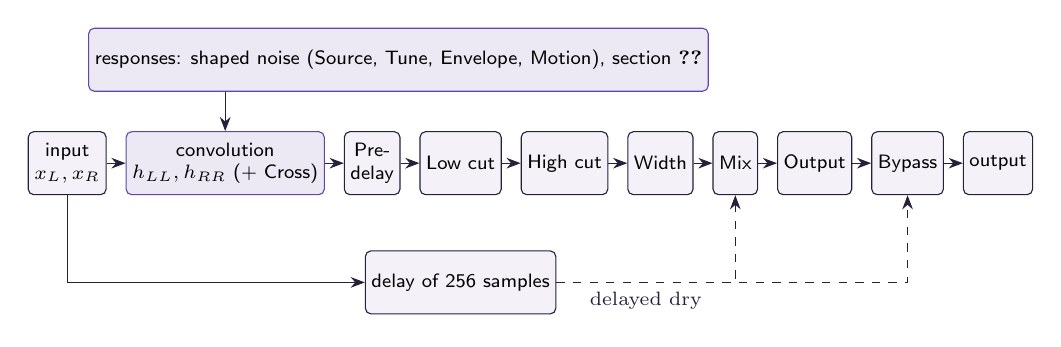
\begin{tikzpicture}[
  node distance=4mm and 2.4mm,
  blk/.style={draw=ink, rounded corners=2pt, fill=paper, minimum height=8mm, align=center,
              font=\scriptsize\sffamily, inner sep=2.2pt},
  core/.style={blk, fill=violet!12, draw=violet},
  arr/.style={-{Stealth[length=1.8mm]}, ink}]
\node[blk] (in) {input\\$x_L, x_R$};
\node[core, right=of in] (conv) {convolution\\$h_{LL}, h_{RR}$ (+ Cross)};
\node[blk, right=of conv] (pd) {Pre-\\delay};
\node[blk, right=of pd] (lc) {Low cut};
\node[blk, right=of lc] (hc) {High cut};
\node[blk, right=of hc] (wd) {Width};
\node[blk, right=of wd] (mix) {Mix};
\node[blk, right=of mix] (out) {Output};
\node[blk, right=of out] (byp) {Bypass};
\node[blk, right=of byp] (s) {output};
\node[core, above=5mm of conv, xshift=22mm] (ir) {responses: shaped noise (Source, Tune, Envelope, Motion), section~\ref{sec:response}};
\node[blk, below=7mm of lc] (dly) {delay of 256 samples};
\draw[arr] (in) -- (conv); \draw[arr] (conv) -- (pd); \draw[arr] (pd) -- (lc); \draw[arr] (lc) -- (hc);
\draw[arr] (hc) -- (wd); \draw[arr] (wd) -- (mix); \draw[arr] (mix) -- (out);
\draw[arr] (out) -- (byp); \draw[arr] (byp) -- (s);
\draw[arr] (ir.south -| conv) -- (conv);
\draw[arr] (in.south) |- (dly.west);
\draw[arr, dashed] (dly.east) -| node[pos=0.25, below, font=\scriptsize] {delayed dry} (mix.south);
\draw[arr, dashed] (dly.east) -| (byp.south);
\end{tikzpicture}
\end{center}

Each output $o$ receives its input convolved with the direct response ($h_{LL}$ on the left,
$h_{RR}$ on the right) and, with Cross, the other input convolved with a crossed response
($h_{RL}$, $h_{LR}$). The dry sound is delayed by the latency of the convolution, 256 samples, to
stay aligned with the pad; the bypass returns this same delayed dry sound, so that the latency does
not change when switching.

\subsection{The impulse responses}\label{sec:response}

The plugin makes two responses (direct paths), or four with Cross, each of
$N = \mathrm{round}(\text{Length} \cdot f_s)$ samples, from an independent noise (seed Seed and
number of the path). Each goes through the following steps.

\begin{enumerate}
\item \textbf{Source.} Gaussian noise of variance 1 (Box-Muller method on the SplitMix64 generator,
  written in the plugin: the same seed gives the same samples on Windows and on Linux); or, if
  Density is below its maximum, sparse noise: in each interval of $f_s$/Density samples, one
  impulse of random sign at a random place, of amplitude $\sqrt{f_s/\text{Density}}$ (power 1).
\item \textbf{Colour.} The spectrum (FFT over the next power of 2) is multiplied by
  \[ \left(\max(f, 20\,\text{Hz}) / 1\,\text{kHz}\right)^{\text{Colour}/6.02}, \]
  the DC component set to zero: the power follows the slope Colour in dB per octave
  (figure~\ref{fig:spectrum}).
\item \textbf{Combs} (Tune). For each note (one with COMB, those of the chord with CHORD):
  $y(n) = x(n) + g\, y(n - D)$, $D = f_s / f$ (linear interpolation), $f = f_0 \cdot 2^{\,\text{Vibrato}
  \cdot \sin(2\pi\, \text{LFO rate}\; t)/12}$, $g = 10^{-3 D / (f_s T_{60})}$ with $T_{60}$ the ring
  time; the outputs of the combs are summed. The combs run on a noise started $\min(T_{60},
  5\,\text{s})$ before $t = 0$, so that they ring steadily from the start.
\item \textbf{Envelope.} Without Damping, Bloom or LFO tone, the envelope $e(t)$ is applied in time
  (rise $\sin^2$ up to $T_a$ = Swell $\cdot$ Length, then a straight line in dB down to Decay).
  Otherwise it depends on frequency and is applied by a short-time Fourier transform (square-root
  Hann windows of 2048 samples at 48\,kHz, overlap of 3/4): for each frame and each frequency, the
  gain of the envelope with a peak at $T_a(f) = T_a + \text{Bloom} \cdot \frac{L}{2} \cdot u(f)$,
  $u(f) = \log_2(f / 1\,\text{kHz})/4$ bounded to $[-1, 1]$, an end level $\text{Decay} -
  \text{Damping} \cdot \max(0, \log_2(f / 250\,\text{Hz}))$, and the colour factor of the LFO
  $(\max(f, 20) / 1000)^{\,\text{LFO tone} \cdot \sin(2\pi\, \text{LFO rate}\; t)/6.02}$. Then, in
  both cases, the $\cos^2$ fade over the last $\min(20\,\text{ms}, L/10)$.
\item \textbf{Rhythm.} Gate of period $T$ = (length of the division) $\times\, 60$ / tempo; each
  step $k$, from $kT$: $\sin^2$ rise over $\min(\max(\text{Attack}\cdot T, 1\,\text{ms}),
  \text{Duty}\cdot T)$, held until $\text{Duty}\cdot T$, $\cos^2$ fall over $\max(\text{Release}\cdot T,
  1\,\text{ms})$; the gate is the largest of the levels of the current step and of the falls of the
  previous ones. With Duty 100\,\% and no Attack, it stays open.
\item \textbf{Normalisation.} Energy 1: $\sum_n h(n)^2 = 1$.
\end{enumerate}
Then output $o$ is made of the direct path $\times \cos(c\,\pi/4)$ and the crossed path $\times
\sin(c\,\pi/4)$, $c$ = Cross: an input with independent channels keeps its level. Last, the stereo
motion multiplies the left output by $\sqrt{2} \cos a$ and the right one by $\sqrt{2} \sin a$,
$a = \frac{\pi}{4}(1 + \text{Pan depth} \cdot \sin(2\pi\, \text{Pan rate}\; t))$.

For a broadband input little correlated in time, the pad thus keeps the RMS level of the input,
whatever the settings. An isolated note, on the other hand, is smeared: its peak falls all the
more as the response is long, its energy is kept.

The streams are computed in parallel, in threads of the plugin. A rebuild takes 0.02\,s with the
default settings; in the worst case (10\,s, a chord of four notes, every treatment, Cross),
0.26\,s at 48\,kHz and 1.05\,s at 192\,kHz. Each treatment is checked by the tests on the
responses made, against its law (colour within 0.7\dB{} per octave, damping within 0.8\dB, bloom
within 0.15\,s, vibrato within 0.4\,Hz\ldots).

\begin{figure}[htbp]
\centering
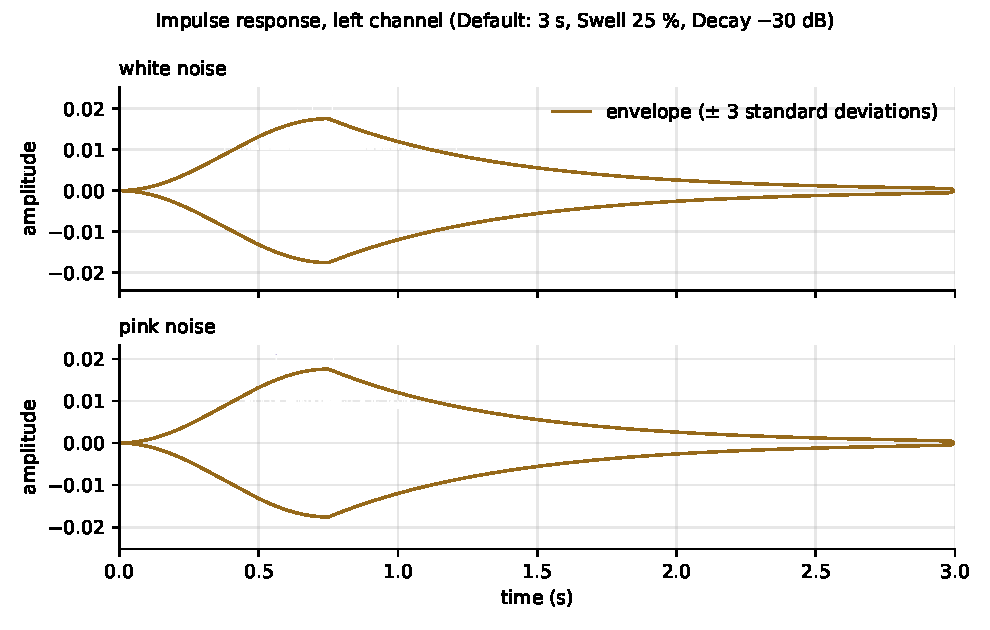
\includegraphics[width=\textwidth]{fig_reponse_en.pdf}
\caption{Response of the Default preset, left channel, with white and with pink noise, and its
envelope.}
\label{fig:response}
\end{figure}

\begin{figure}[htbp]
\centering
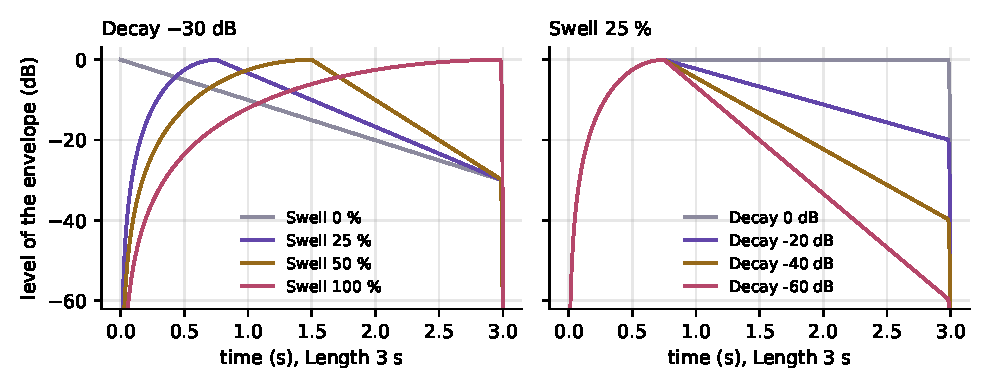
\includegraphics[width=\textwidth]{fig_enveloppes_en.pdf}
\caption{Envelope for a length of 3\,s: effect of Swell (left) and of Decay (right).}
\label{fig:envelopes}
\end{figure}

\begin{figure}[htbp]
\centering
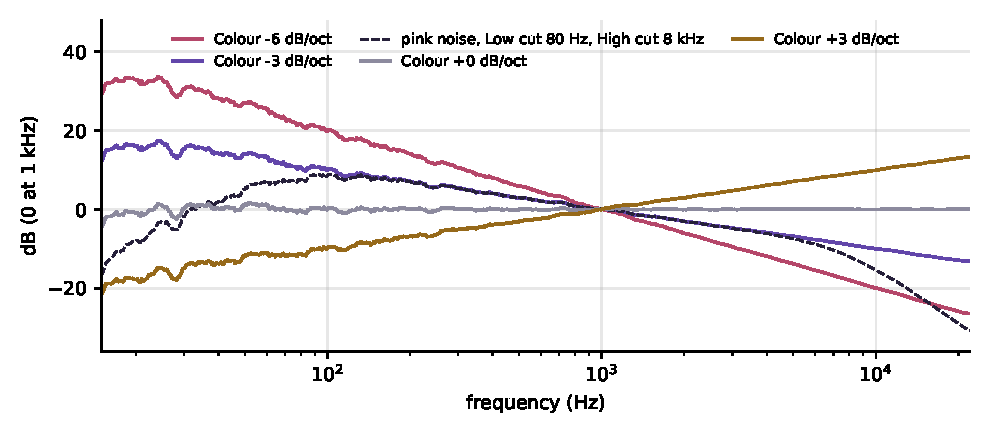
\includegraphics[width=\textwidth]{fig_spectre_en.pdf}
\caption{Spectrum of the response against Colour (mean of both channels, 4\,s, flat envelope),
measured on the responses of the plugin and smoothed over a sixth of an octave; dashed, pink noise
with Low cut 80\,Hz and High cut 8\,kHz.}
\label{fig:spectrum}
\end{figure}

\begin{figure}[htbp]
\centering
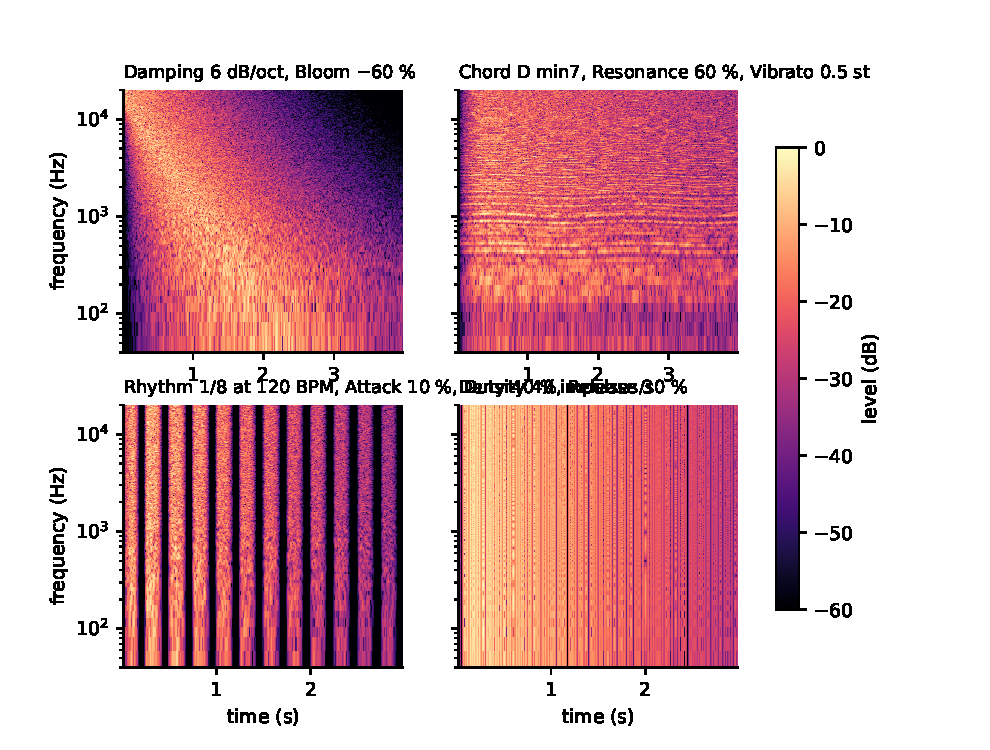
\includegraphics[width=\textwidth]{fig_traitements_en.pdf}
\caption{Time-frequency maps of responses of the plugin (white noise): Damping and Bloom (the highs
arrive early and die soon), chord with vibrato (the harmonics of the four notes waver), rhythmic
gate, sparse noise (isolated impulses).}
\label{fig:treatments}
\end{figure}

\begin{figure}[htbp]
\centering
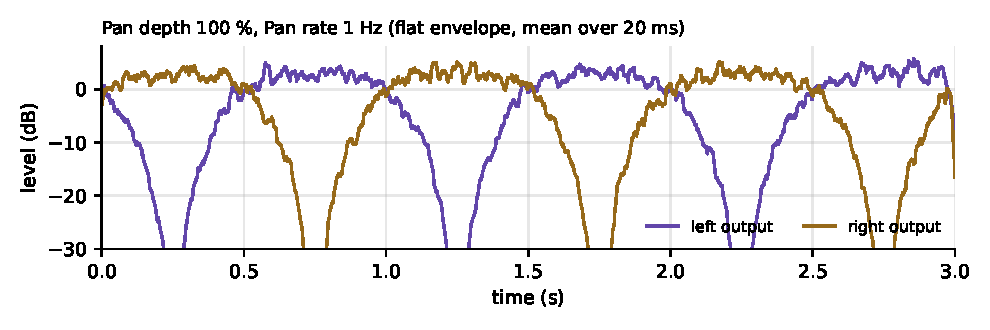
\includegraphics[width=\textwidth]{fig_stereo_en.pdf}
\caption{Stereo motion: level of the left and right outputs along the response.}
\label{fig:stereo}
\end{figure}

\subsection{The convolution}\label{sec:convolution}

A 10\,s response at 48\,kHz holds 480\,000 samples: direct convolution would cost nearly a billion
multiplications per second and per channel. The plugin computes it in the frequency domain, by
blocks (\emph{uniformly partitioned convolution}, overlap-save, real FFTs of pffft), in two stages:

\begin{center}
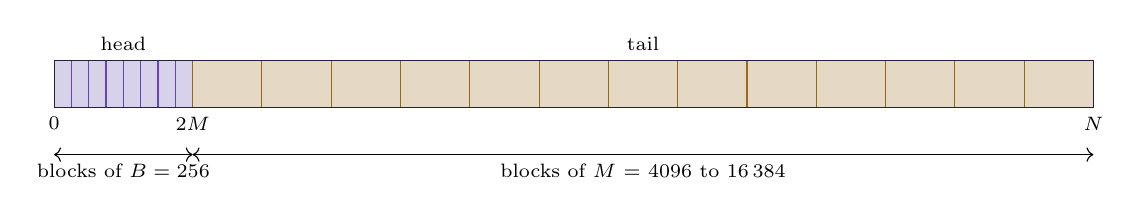
\begin{tikzpicture}[x=0.55mm, y=1mm]
\fill[violet!25] (0,0) rectangle (32,6);
\foreach \i in {0,4,...,28} \draw[violet] (\i,0) rectangle (\i+4,6);
\fill[amber!25] (32,0) rectangle (240,6);
\foreach \i in {32,48,...,224} \draw[amber] (\i,0) rectangle (\i+16,6);
\draw[ink] (0,0) rectangle (240,6);
\node[font=\scriptsize, above] at (16,6) {head};
\node[font=\scriptsize, above] at (136,6) {tail};
\node[font=\scriptsize, below] at (0,0) {0};
\node[font=\scriptsize, below] at (32,0) {$2M$};
\node[font=\scriptsize, below] at (240,0) {$N$};
\draw[<->] (0,-6) -- node[below, font=\scriptsize] {blocks of $B = 256$} (32,-6);
\draw[<->] (32,-6) -- node[below, font=\scriptsize] {blocks of $M$ = 4096 to 16\,384} (240,-6);
\end{tikzpicture}
\end{center}

\begin{itemize}
\item \textbf{Head}: the first $2M$ samples of the response, in blocks of $B = 256$. For each block
  of 256 input samples: one 512-point FFT, one product per block of the response, one inverse FFT.
  This stage sets the latency: 256 samples.
\item \textbf{Tail}: the rest, in blocks of $M$ = 4096 samples ($f_s \leq 50$\,kHz), 8192
  ($\leq 100$\,kHz) or 16\,384. Block $j$ of the input only acts on the output from sample
  $jM + 2M$ on: the plugin thus has $M$ samples of time to compute its contribution (one FFT, the
  products with all the blocks of the tail, one inverse FFT) and spreads it evenly over the $M/B$
  blocks of 256 before. There is neither a peak of computation nor an extra thread in the audio
  processing.
\end{itemize}
Both stages share the spectra of the input already computed (frequency-domain delay lines); with
Cross, each output adds the products of the crossed responses with the spectra of the other input,
which doubles the products without any further transform. The
result is that of the exact convolution, up to the rounding of single-precision computation: the
tests compare it with a direct convolution in double precision, with a deviation of at most
$4.4 \cdot 10^{-7}$ of the peak, for responses from 1 sample to $5M$ and at 48, 96 and 192\,kHz,
and of $3.5 \cdot 10^{-7}$ with the crossed responses.

\paragraph{Cost.} Measured on one core (blocks of 256, stereo):
\begin{center}
\small
\begin{tabular}{@{}l r r r@{}}
\toprule
Length & 48\,kHz & 96\,kHz & 192\,kHz \\
\midrule
3\,s  & 1.0\,\% & 3.0\,\% & 8.8\,\% \\
10\,s & 2.2\,\% & 5.4\,\% & 15\,\% \\
10\,s, Cross & 4.5\,\% & 10\,\% & 25\,\% \\
\bottomrule
\end{tabular}
\end{center}
The treatments of the noise cost nothing during playback: they are in the response. The memory used
is about 20\,MB at 48\,kHz (40\,MB with Cross); during a rebuild, computing the response briefly
needs more (up to 340\,MB in the worst case at 192\,kHz).

\subsection{Change of response}\label{sec:change}

The settings of the SOURCE, TUNE, ENVELOPE and MOTION sections define the response: changing one
of them means making it again, as does a change of the tempo of the host while RHYTHM is on. A
setting without effect with the others (NOTE when TUNE is OFF, for example) does not. This work is
done in a thread of the plugin, never in the audio processing, which goes on with the old response.
When the new one is ready, it is taken at the start of a tail block. Since the spectra of the input
do not depend on the response, the new response has the whole past of the signal at once: the pad
does not start again from silence. The output goes from the old response to the new one by a linear
crossfade of $M$ samples (85\,ms at 48\,kHz), then the old one is freed, in the thread of the
plugin.

Turning one of these knobs during playback therefore gives a series of crossfades, without a click,
with a slight delay. When the plugin is activated (start of playback or of a render), the response
is built at once: a render always starts with the right response.

\subsection{Pre-delay, width, filters, mix and output}

\paragraph{Pre-delay.} Integer delay of the pad in samples, right after the convolution; a change
crossfades from the old delay to the new one in 30\,ms, the next change waits for the end of the
crossfade.

\paragraph{Filters.} Low cut and High cut are second-order Butterworth filters (Robert
Bristow-Johnson's formulas), in double precision; their frequency is limited to 0.45\,$f_s$.
When off, their coefficients are those of the identity: the output is then exactly the input.

\paragraph{Width.} On the pad: $m = (p_L + p_R)/2$, $s = (p_L - p_R)/2 \cdot$ Width,
$p_L' = m + s$, $p_R' = m - s$.

\begin{figure}[htbp]
\centering
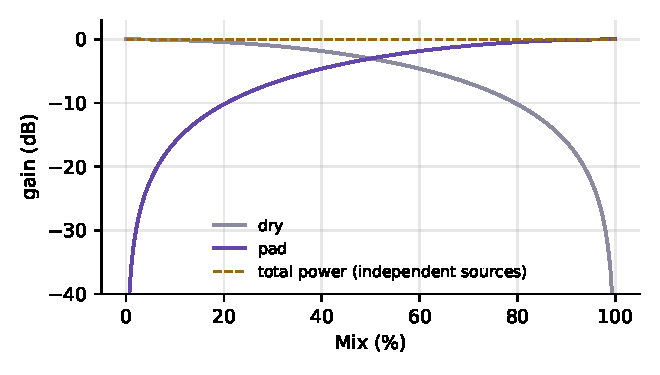
\includegraphics[width=0.6\textwidth]{fig_mix_en.pdf}
\caption{Law of the mix: gains of the dry sound and of the pad against Mix.}
\label{fig:mix}
\end{figure}

\paragraph{Mix and output.} $y = (\text{pad} \cdot \sin(\tfrac{\pi}{2} m) + \text{delayed dry}
\cdot \cos(\tfrac{\pi}{2} m)) \cdot g$, $g$ = gain of Output; the gains are exactly 0 and 1 at
both ends of Mix.

\subsection{Smoothing of the settings and bypass}\label{sec:smoothing}

Mix, Width, Output and the coefficients of both filters go linearly to their new value in 20\,ms,
then take it exactly: no zipper noise when they are turned or automated. The settings of the
response change by crossfade (section~\ref{sec:change}).

\paragraph{Bypass.} The output becomes the dry sound delayed by 256 samples, exactly, through a
10\,ms crossfade; the latency stays the same. The convolution keeps running during the bypass, so
that the pad is already there when it is released.

\subsection{Denormal numbers}

In silence, the states of the filters decay towards zero and would go through denormal numbers,
very slow on x86. The plugin switches the FTZ/DAZ modes of the processor on for the time of its
computation and gives the host its own state back on return.

% ==============================================================================================
\section{Tips}

\begin{description}
\item[A pad from an instrument.] Soft pad or Endless wash on an auxiliary send, Mix at 100\,\%:
  detached notes become a continuous background. The longer the Length and the closer Decay is to
  0, the steadier the pad.
\item[A tuned pad.] Tuned drone or Chord pad on a rich source (drums, noise, distorted guitar): the
  pad takes the note or the chord. Tune NOTE to the key of the song; raise RESONANCE for clearer
  notes.
\item[Thickening.] Short smear (0.4\,s) on a voice, a guitar or a snare: the sound gets a dense
  tail, without the space of a reverb.
\item[Swells.] Reverse swell: each attack rises for 2\,s and then stops short. With a send placed
  a few beats before, the swell leads into the sound.
\item[Rhythm.] Pulse gate: the pad pulses in eighth notes on the tempo; short DUTY, ATTACK and
  RELEASE for crisp rhythmic echoes, long edges for breathing.
\item[Realism.] DAMPING 3 to 6\dB/oct makes the tail more natural; a negative BLOOM gives a pad
  that warms up as it settles.
\item[Low end.] Pink and brown noise give a lot of low end: Low cut 60 to 150\,Hz, especially on a
  send shared by several tracks.
\item[Hiss.] White or blue noise makes a hiss audible on soft sounds: High cut between 6 and
  12\,kHz, or a lower colour.
\item[Texture.] If one frequency stands out too much on a sustained sound, change Seed.
\item[Mono.] The pad is very wide; check in mono and reduce Width if the mix gets hollow.
\item[Comparing two settings.] Set A, copy it to B (\ctl{A>B}), change B, then switch A | B.
\end{description}

\section{Files, projects and compatibility}\label{sec:files}

\begin{description}
\item[With the project.] All the settings and the inactive A/B set (state \texttt{ab}). The
  settings are read back by their names: adding a setting in a future version does not break a
  project. The response is not saved: it is made again, identical, from the settings.
\item[On the computer.] The theme in \texttt{padifier.conf} (\texttt{theme=dusk} or
  \texttt{pearl}) and your presets in \texttt{presets/}, one file \texttt{<name>.preset} each, in
  the folder:
  \begin{itemize}
  \item Windows: \verb|%APPDATA%\Padifier\|;
  \item Linux: \verb|$XDG_CONFIG_HOME/padifier/|, otherwise \verb|~/.config/padifier/|.
  \end{itemize}
\item[Format of a preset.] Text, one line \texttt{key=value} per setting (the symbols of the
  parameters: \texttt{colour}, \texttt{length}, \texttt{swell}, \texttt{decay}, \texttt{seed},
  \texttt{density}, \texttt{tune}, \texttt{note}, \texttt{chord}, \texttt{resonance},
  \texttt{damping}, \texttt{bloom}, \texttt{lforate}, \texttt{lfopitch}, \texttt{lfotone},
  \texttt{rhythm}, \texttt{attack}, \texttt{duty}, \texttt{release}, \texttt{panrate}, \texttt{pandepth}, \texttt{cross},
  \texttt{predelay}, \texttt{lowcut}, \texttt{highcut}, \texttt{width}, \texttt{mix},
  \texttt{output}), numbers with a decimal point whatever the language of the system. A missing
  key takes its default value, a value out of range is brought back within the range, an unknown
  line is ignored. Copying the file is enough to share a preset.
\item[From 1.0.] The Noise setting (white or pink) became Colour: a project or a preset of 1.0 keeps
  its other settings, the colour goes back to pink ($-3$) and the new settings to their defaults,
  so that the sound is that of 1.0 with pink noise.
\end{description}

% ==============================================================================================
\section{Known limits}\label{sec:limits}
\begin{itemize}
\item Latency of 256 samples: compensated by the host, but audible when playing live through the
  plugin with a very small buffer.
\item A change of the settings of the response arrives with a slight delay (the time to make it
  again, up to 1\,s in the worst case at 192\,kHz); in an offline render faster than real time, an
  automation of these settings may therefore land a little later than on playback.
\item The motions (LFO, rhythm, stereo) start at the attack of each sound, not on the time of the
  song.
\item The convolution creates no frequency: TUNE brings out what the source contains near the
  notes, it transposes nothing.
\item The pad has no freeze: it always follows the input.
\item Typing on the keyboard (values, preset names) depends on the host: some keep the keyboard
  for themselves.
\item The host only sees the factory presets.
\end{itemize}

% ==============================================================================================
\section{Credits}
FFT: pffft, Julien Pommier, after FFTPACK (Paul Swarztrauber, NCAR). Pseudo-random generator:
SplitMix64 (Steele, Lea and Flood, 2014). Filters: Robert Bristow-Johnson's formulas (\emph{Audio
EQ Cookbook}). Plugin framework and interface: DPF (DISTRHO Plugin Framework, ISC), with NanoVG
(zlib), pugl (ISC), the CLAP headers (MIT) and the DejaVu Sans font. The licence notices of these
components are in \texttt{THIRD\_PARTY\_LICENSES.txt}, installed with the plugin and included in
every archive.

\end{document}
